\chapter{Исследовательский раздел}
\section{Условия исследований}
Исследование проводилось на компьютере со следующими характеристиками:

\begin{itemize}
\item 8-ядерный процессор 11th Gen Intel Core i7-1165G7;
\item операционная система Linux (дистрибутив Ubuntu 20.04.5 LTS, версия ядра Linux 5.15.0-56, архитектура x86-64);
\item 16 Гб оперативной памяти.
\end{itemize}

Для динамического анализа информации о процессах была разработана программа, выводящая информацию из файла /proc/analyzer заданное количество раз с интервалом времени в 1 секунду. 

Для получения идентификатора исследуемого процесса использовалась утилита lsof \cite{bib:2}. 

Для фильтрации вывода разработанной программы по идентификатору процесса использовались утилиты awk и grep \cite{bib:2}.

\section{Исследование процесса проигрывания ау\-диофайла}

На рисунке \ref{audio} представлен вывод команд lsof и разработанной программы. Так как приоритет процесса равен 120, можно сделать вывод, что процесс проигрывания аудиофайла был запланирован как обычный процесс (не процесс реального времени).

\begin{figure}[H]
	\centering
	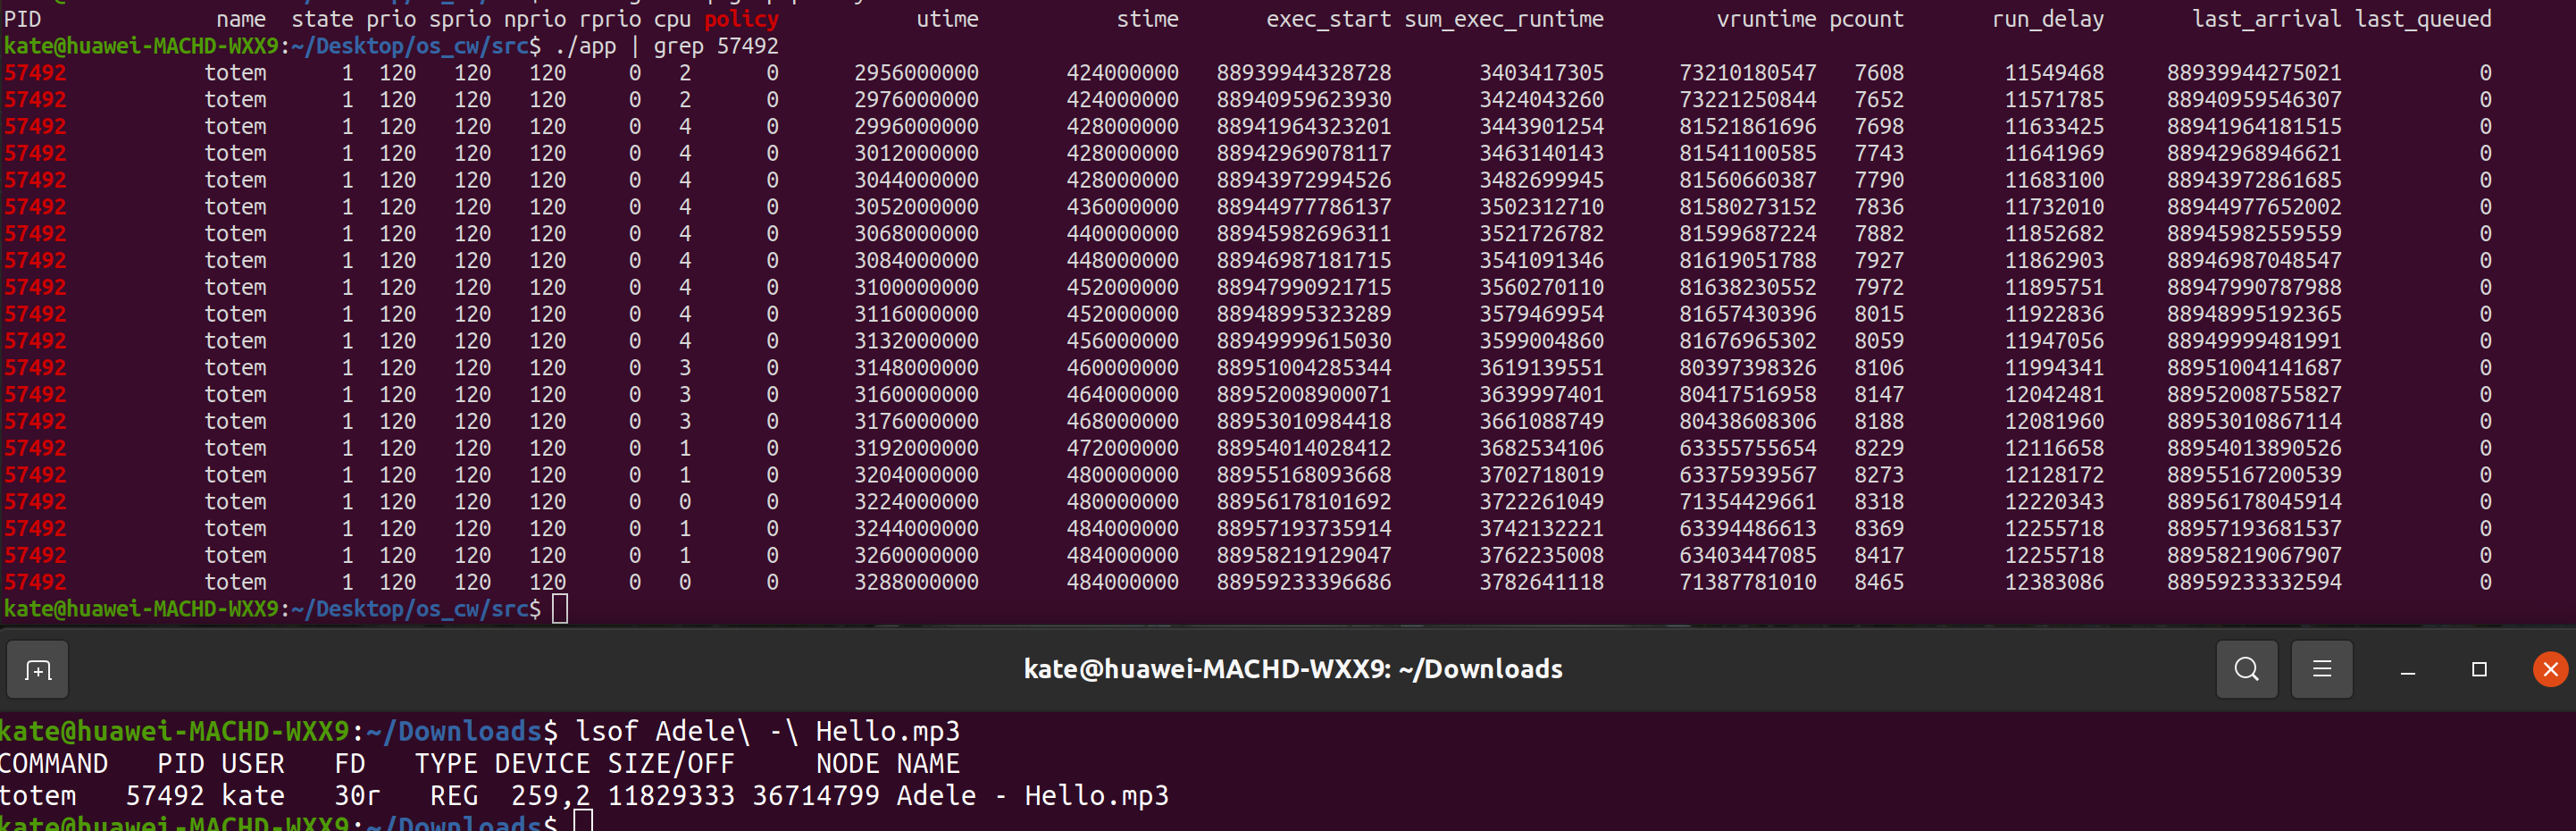
\includegraphics[width=\linewidth]{img/audio.png}
	\caption{Вывод программы при проигрывании аудиофайла}
	\label{audio}
\end{figure}

\section{Исследование процесса проигрывания видеофайла}

На рисунке \ref{video} представлен вывод команды lsof и разработанной программы. Так как приоритет процесса равен 120, можно сделать вывод, что процесс проигрывания видеофайла был запланирован как обычный процесс (не процесс реального времени).

\begin{figure}[H]
	\centering
	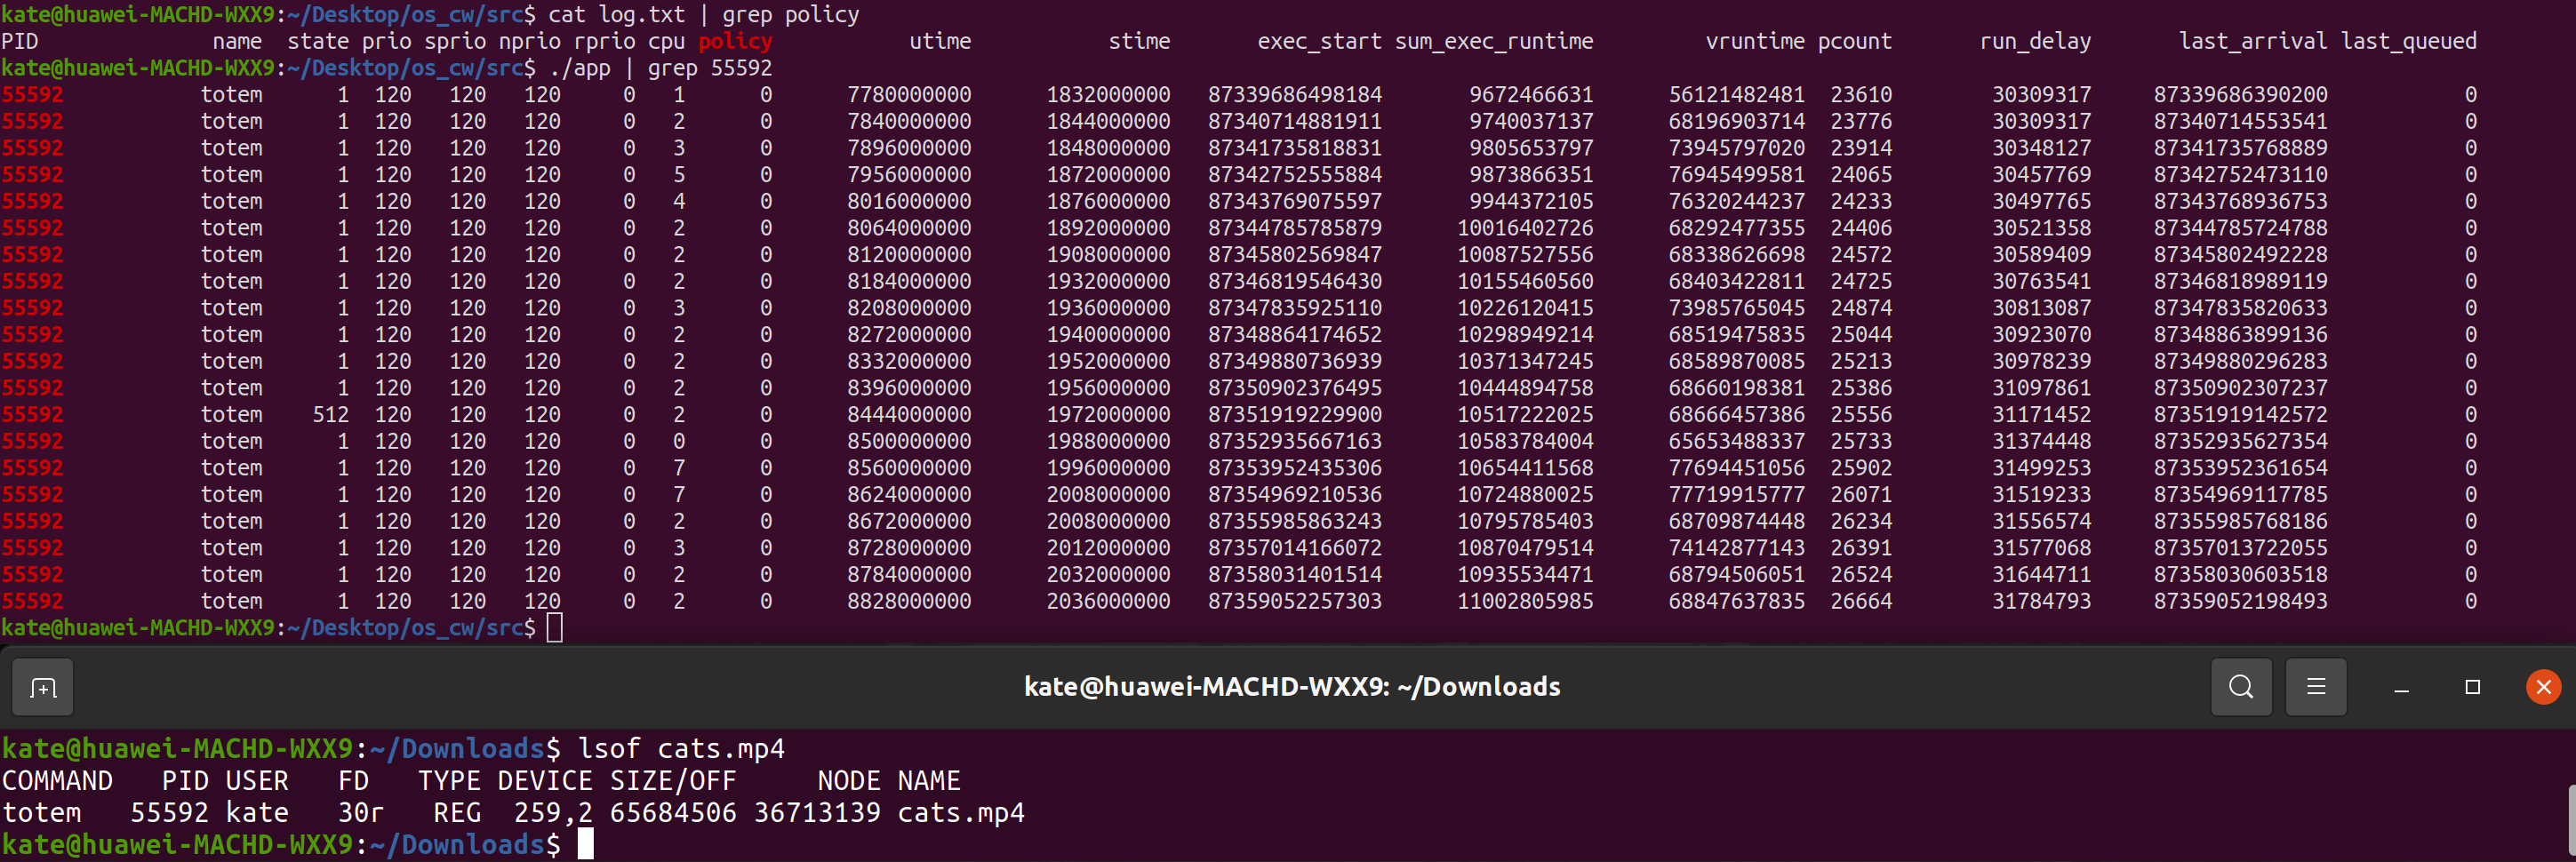
\includegraphics[width=\linewidth]{img/video.png}
	\caption{Вывод программы при проигрывании видеофайла}
	\label{video}
\end{figure}
\newpage
\section{Исследование процесса игры}

На рисунке \ref{game} представлен вывод разработанной программы во время игры. Так как приоритет игрового процесса равен 120, можно сделать вывод, что процесс игры был запланирован как обычный процесс (не процесс реального времени).

\begin{figure}[H]
	\centering
	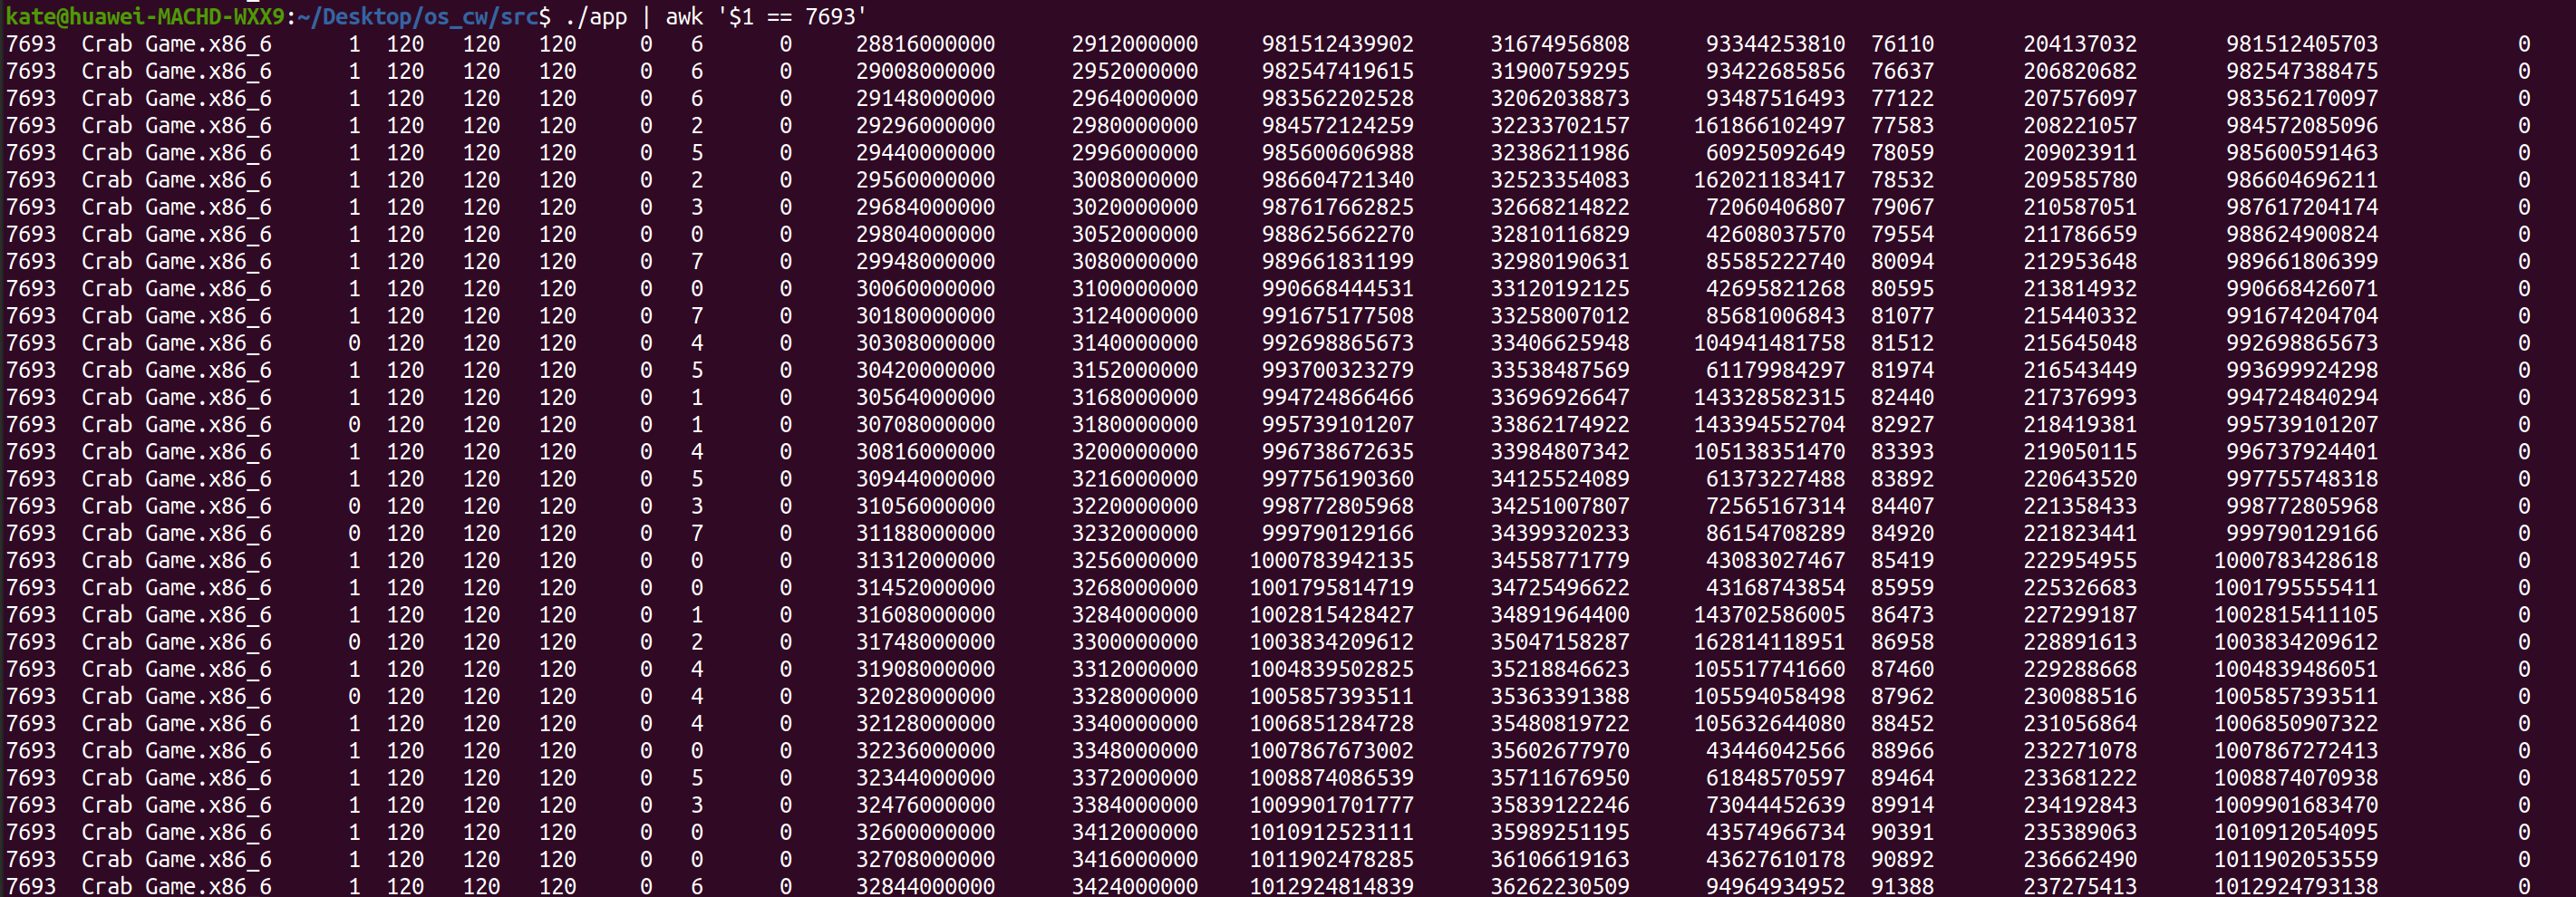
\includegraphics[width=\linewidth]{img/game.png}
	\caption{Вывод программы во время игрового процесса}
	\label{game}
\end{figure}

\section{Исследование интерактивного процесса}
Для проведения исследования дополнительно была разработана программа, которая читает введённые через терминал символы с помощью системного вызова read. Кроме того, был разработан модуль ядра, в котором регистрируется обработчик прерывания на событие на клавиатуре, в котором выводится приоритет исследуемого интерактивного процесса.

% при этом в момент нажатия на клавишу выводится информация из файла /proc/analyzer. 

% Так как язык C не предоставляет возможности обрабатывать сигнал нажатия на клавиши напрямую, этот механизм был реализован в 2 этапа:
% \begin{itemize}
%     \item терминал был переведён из режима <<canonical>> в <<raw>> режим, то есть были отключены функции обработки введённых символов (в том числе построковая, а не посимвольная обработка), отключен режим <<echo>>, отключен таймер на ввод и др. \cite{bib:6};
%     \item для потока ввода был назначен обработчик сигнала SIGIO, который выводит информацию из файла в /proc.
% \end{itemize}

На рисунке \ref{img:interactive} представлен вывод программы интерактивного процесса. Так как приоритет процесса равен 120, можно сделать вывод, что интерактивный процесс был запланирован как обычный процесс (не процесс реального времени).

\begin{figure}[H]
	\centering
	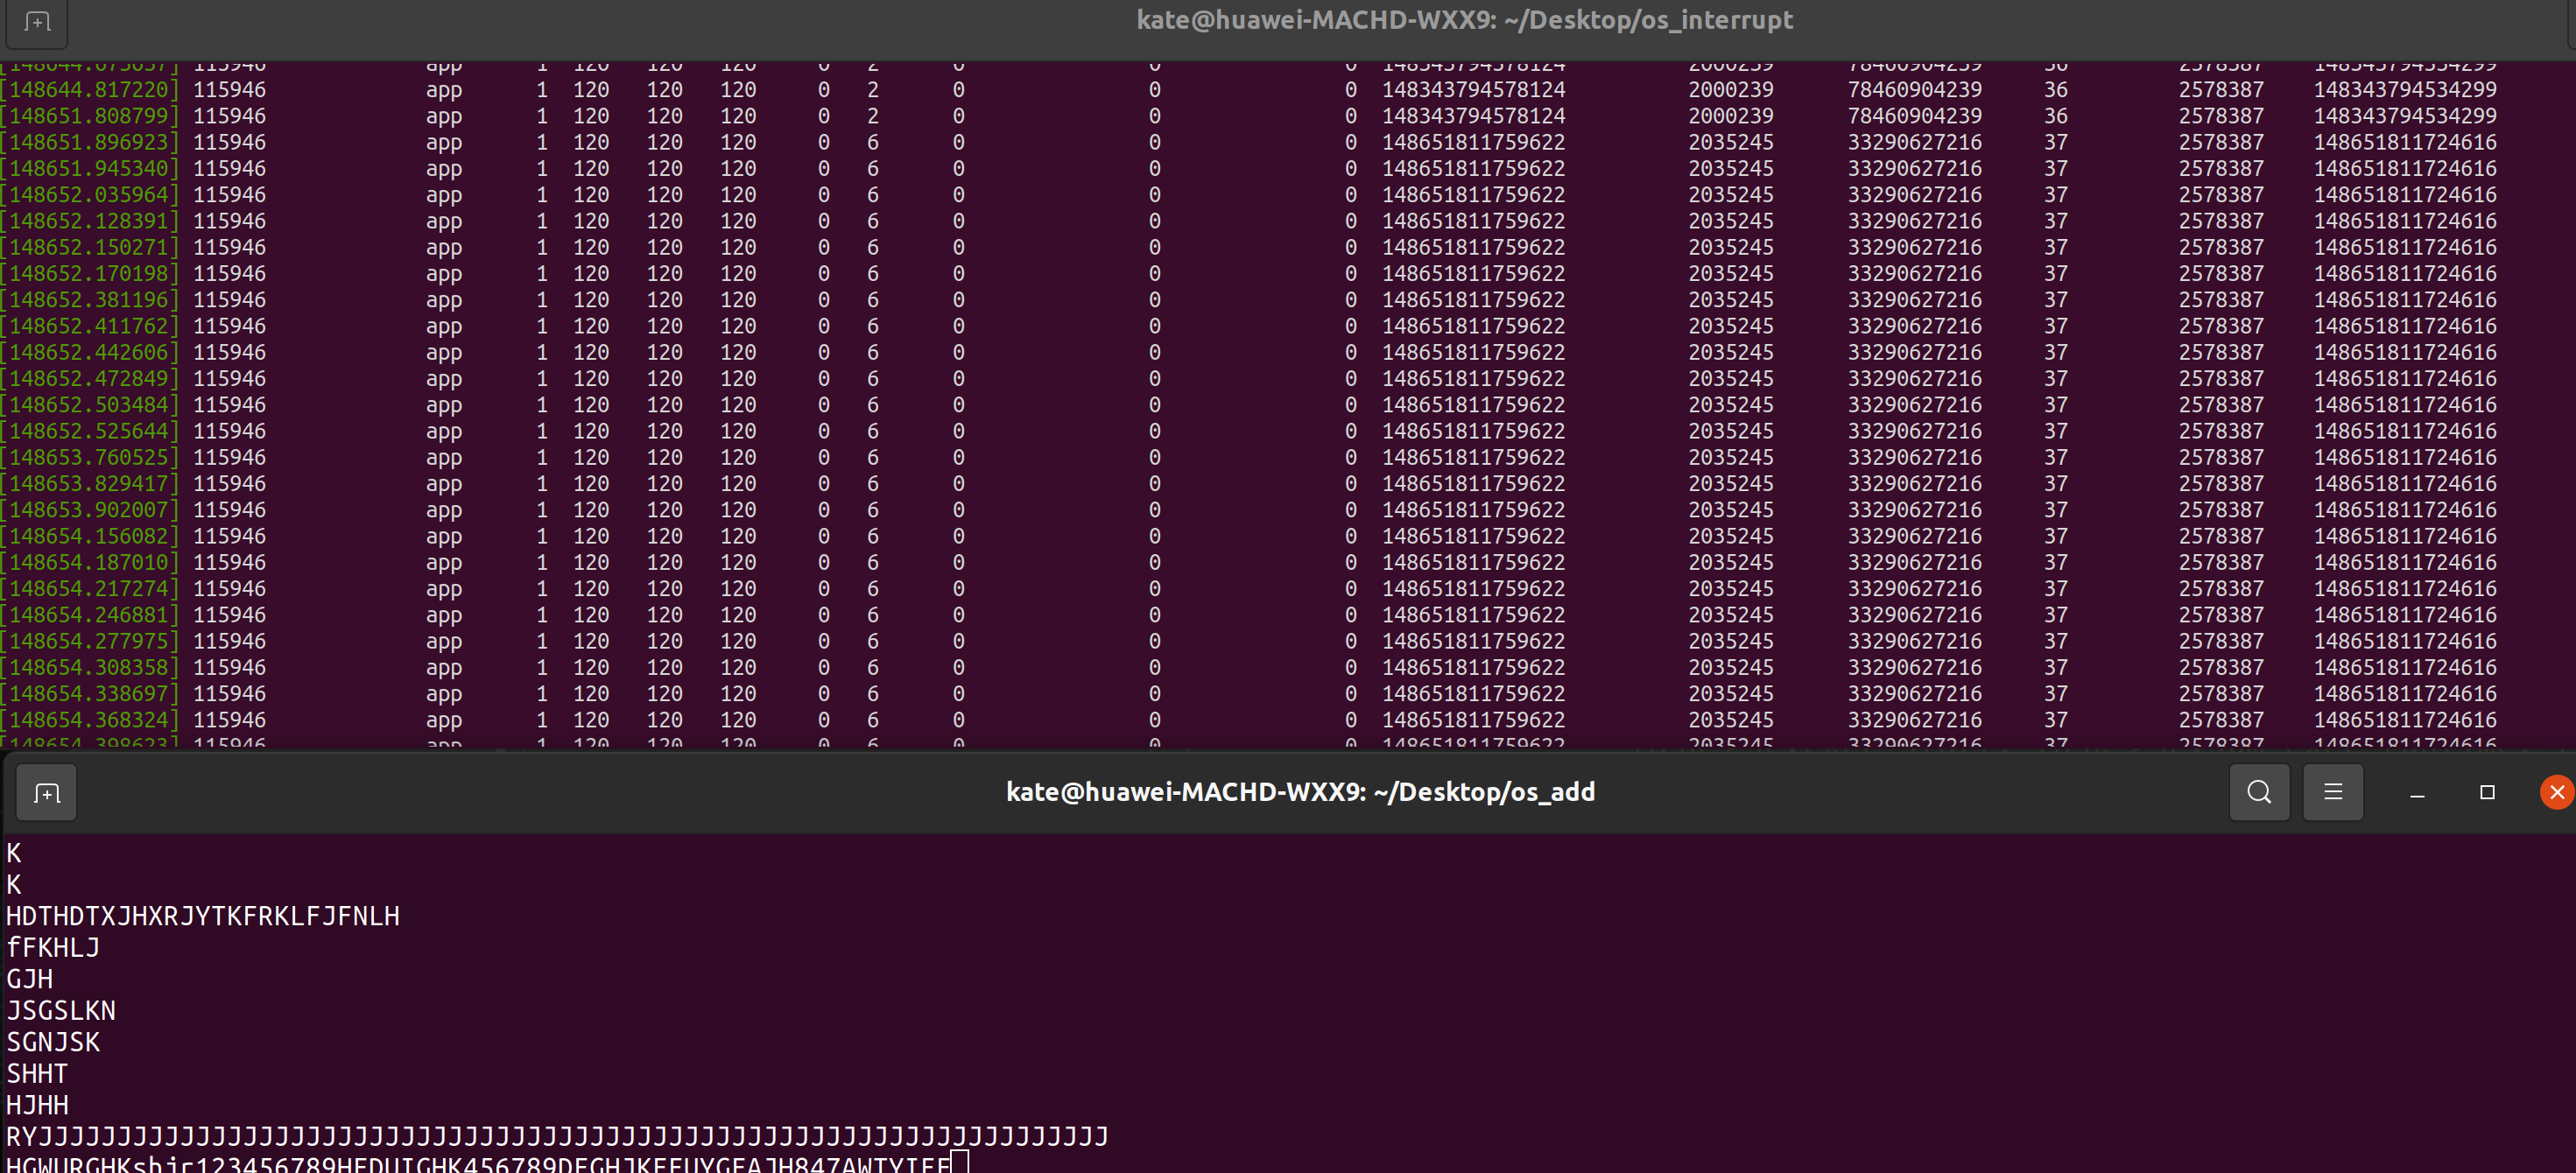
\includegraphics[width=\linewidth]{img/interactive.png}
	\caption{Вывод программы интерактивного процесса}
	\label{img:interactive}
\end{figure}

\section{Исследование ситуации инверсии приоритетов}
Инверсия приоритетов -- ситуация в системе, при которой процесс с высоким приоритетом вынужден ждать выполнение процесса с низким приоритетом. Пусть в системе существуют такие 3 процесса, что: 
\begin{itemize}
    \item процесс A с низким приоритетом;
    \item процесс C с высоким приоритетом;
    \item процесс B со <<средним>> приориетом.
\end{itemize}

Рассмотрим ситуацию, когда процесс A успевает захватить ресурс (мьютекс) раньше процесса C. При этом процесс C после захвата мьютекса может быть вытеснен процессом B из-за более низкого приоритета. Таким образом, процесс A не может выполняться из-за захвата мьютекса процессом C, а процесс C не может выполняться (и отпустить ресурс), так как вытесняется процессом B. Следовательно, высокоприоритетный процесс C ждет выполнение процесса B со средним приоритетом.

Такая ситуация в ядре решается \textbf{временным увеличением} приоритета процесса A до приоритета процесса C до освобождения ресурса. Это называется наследованием приоритетов (priority inheritance).

Для проведения исследования:
\begin{itemize}
    \item был использован код, который создаёт по 3 потока на каждое ядро процессора (с приоритетами 96, 97, 98) и с помощью захвата мьютекса имитирует ситуацию инверсии приоритетов;
    \item был изменён модуль ядра таким образом, чтобы информация выводилась в разрезе потоков, а не процессов;
    \item был изменён код пространства пользователя, который периодически обращается к файлу в /proc, таким образом, чтобы информация выводилась в бесконечном цикле без задержек (чтобы не пропустить изменение приоритетов).
\end{itemize}

На рисунке \ref{img:pi} представлен вывод программы пространства пользователя. На рисунке видно, что процесс 15407 в первой итерации вывода имеет normal\_prio = 98 и prio = 96, а во второй итерации normal\_prio = 98 и prio = 98. Таким образом, низкоприоритетному процессу был временно повышен приоритет до высокоприоритетного для выхода из ситуации инверсии приоритетов.

\begin{figure}[H]
	\centering
	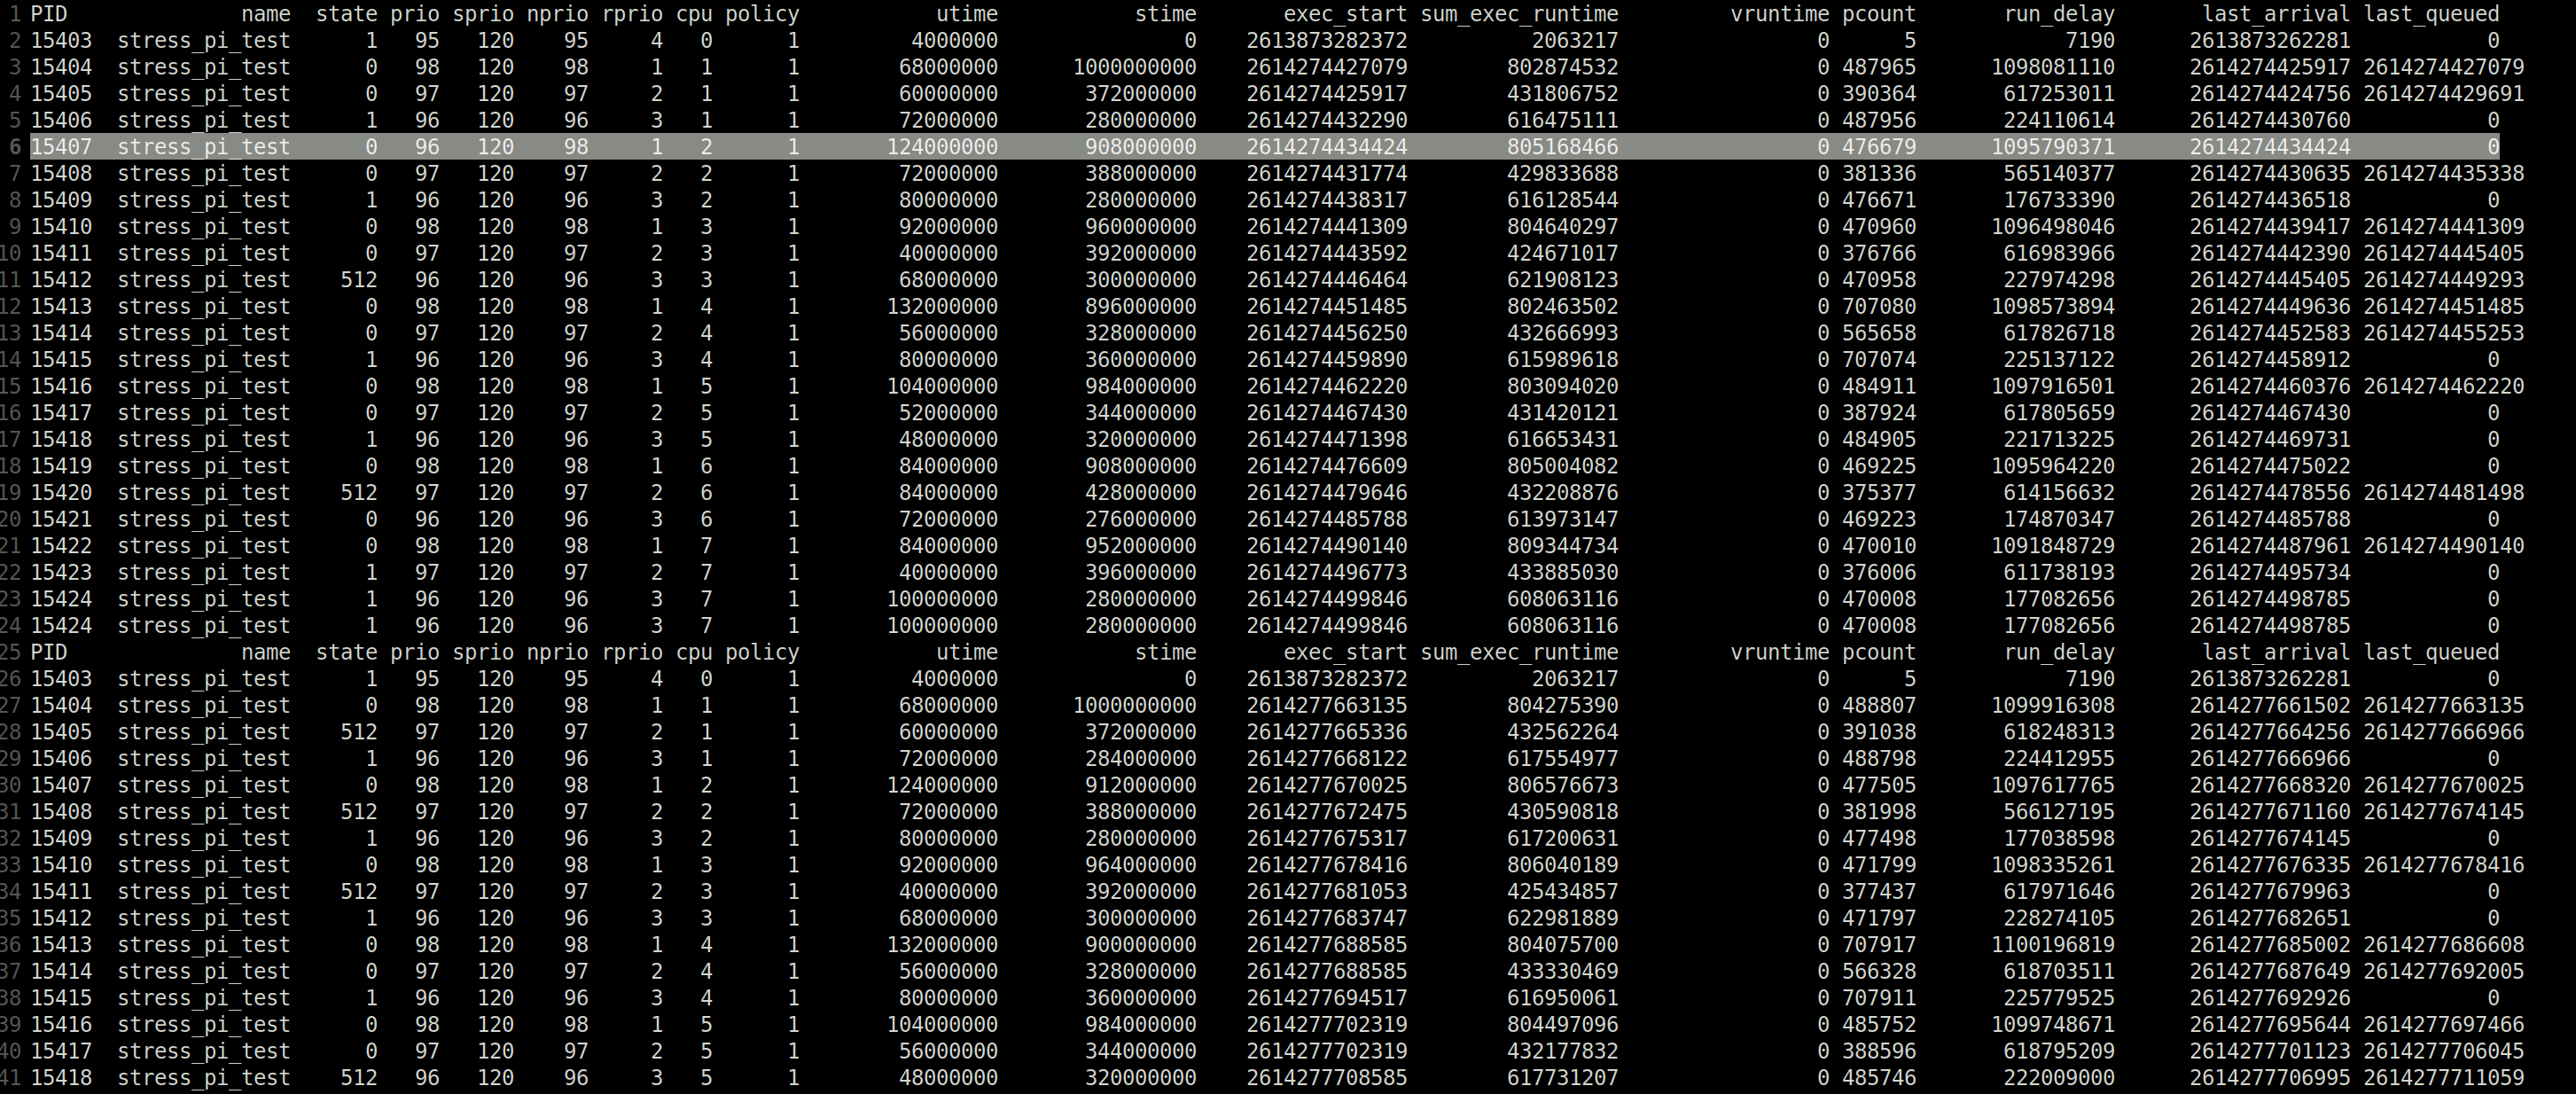
\includegraphics[width=\linewidth]{img/pi.png}
	\caption{Вывод логов в ситуации инверсии приоритетов}
	\label{img:pi}
\end{figure}

\section*{Выводы}
В результате исследований было выяснено, что процессы проигрывания видеофайлов и аудиофайлов, а также игровые и интерактивные процессы в ОС Linux планируются в соответствии с алгоритмом SCHED\_NORMAL и имеют статический приоритет -- 120. Однако в ситуации инверсии приоритетов приоритет низкоприоритетного процесса повышается до приоритета высокоприоритетного процесса. 